\documentclass{article}
\usepackage[utf8]{inputenc}
\usepackage{graphicx}
\usepackage{indentfirst}

\title{Problem Set 6}
\author{Collin DeVore}
\date{March 2023}

\begin{document}

\maketitle

\section*{Question 3}
\indent{For this dataset, there is not much that I had to do to transform and clean the data. The dataset was gathered from Kaggle and is called "Airline Passenger Satisfaction". While it is true that I could have subset the data to get rid of extra columns, or used gsub functions to change the periods to underscores in the column headers, I did not find much need to reformat this for my purposes. I began by checking the head and the tail of the dataset to ensure that the data was read correctly. After this was done, I changed all of the letters in the "satisfaction" column to upper case, since they will be used on the x-axis on the second and third plots. I also changed the " OR " in the satisfaction column to "/" so that the variable looks cleaner.}\\
\indent{For the donut chart, I created a simplified dataframe with the fraction of the individuals who were satisfied and the fraction of the individuals who were either neutral or dissatisfied. I added maximum and minimum values for the chart and labels to make the chart look cleaner. For the bar chart, I created a new variable in the dataframe that consisted of both the satisfaction variable and the cabin class. I then aggregated the data by averaging the flight distance across the new variable values. Finally, the data was fully clean and could be used for each of the plots.}\\

\section*{Question 4}
\noindent{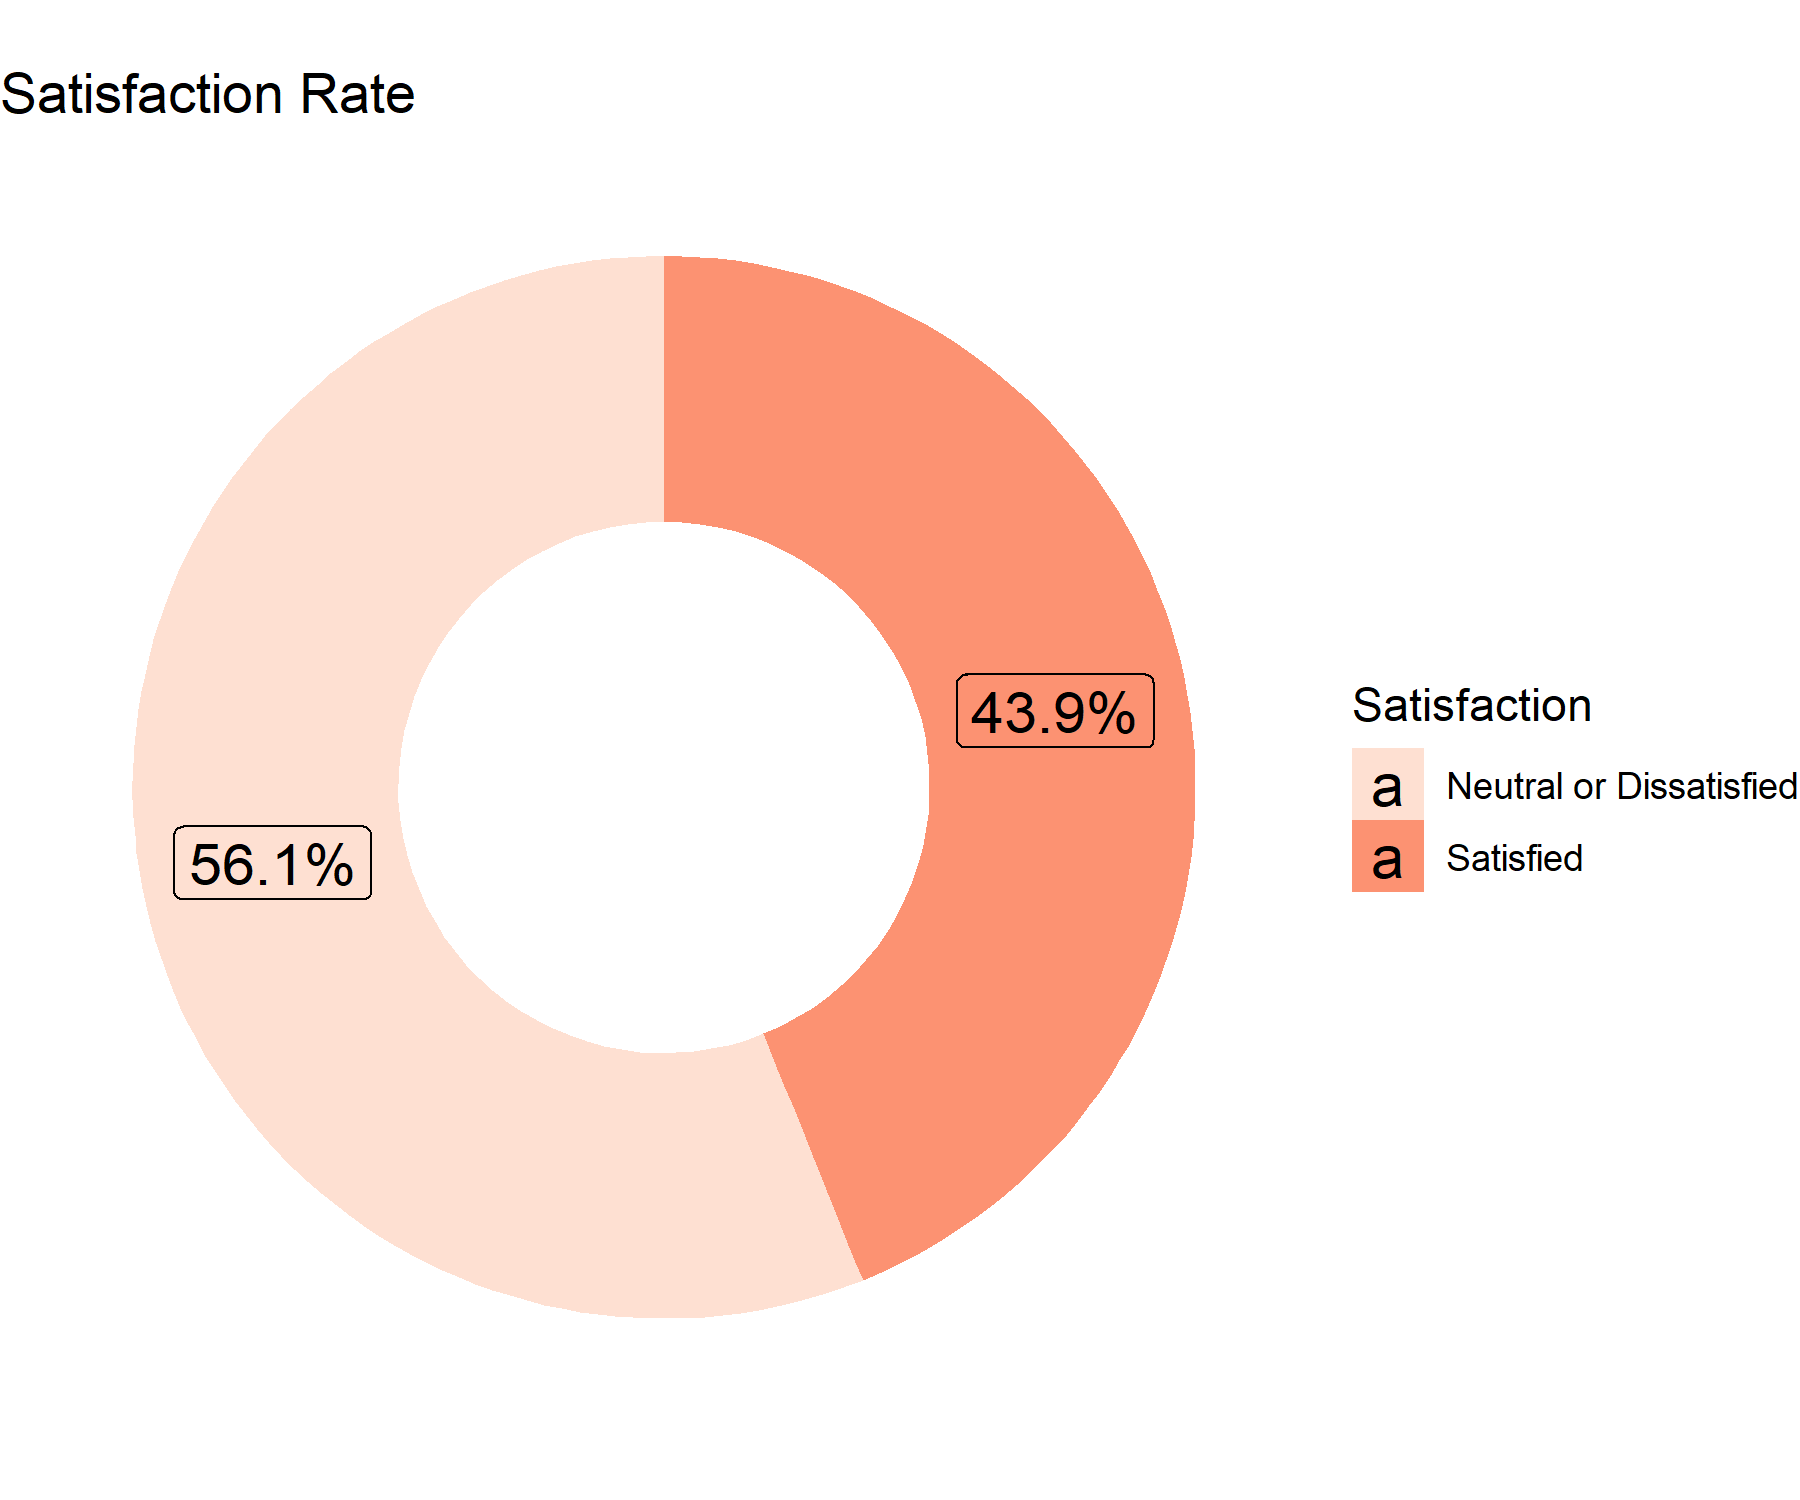
\includegraphics[width = 6in, height = 5in]{PS6a_DeVore.png}}\\
 \\
\noindent{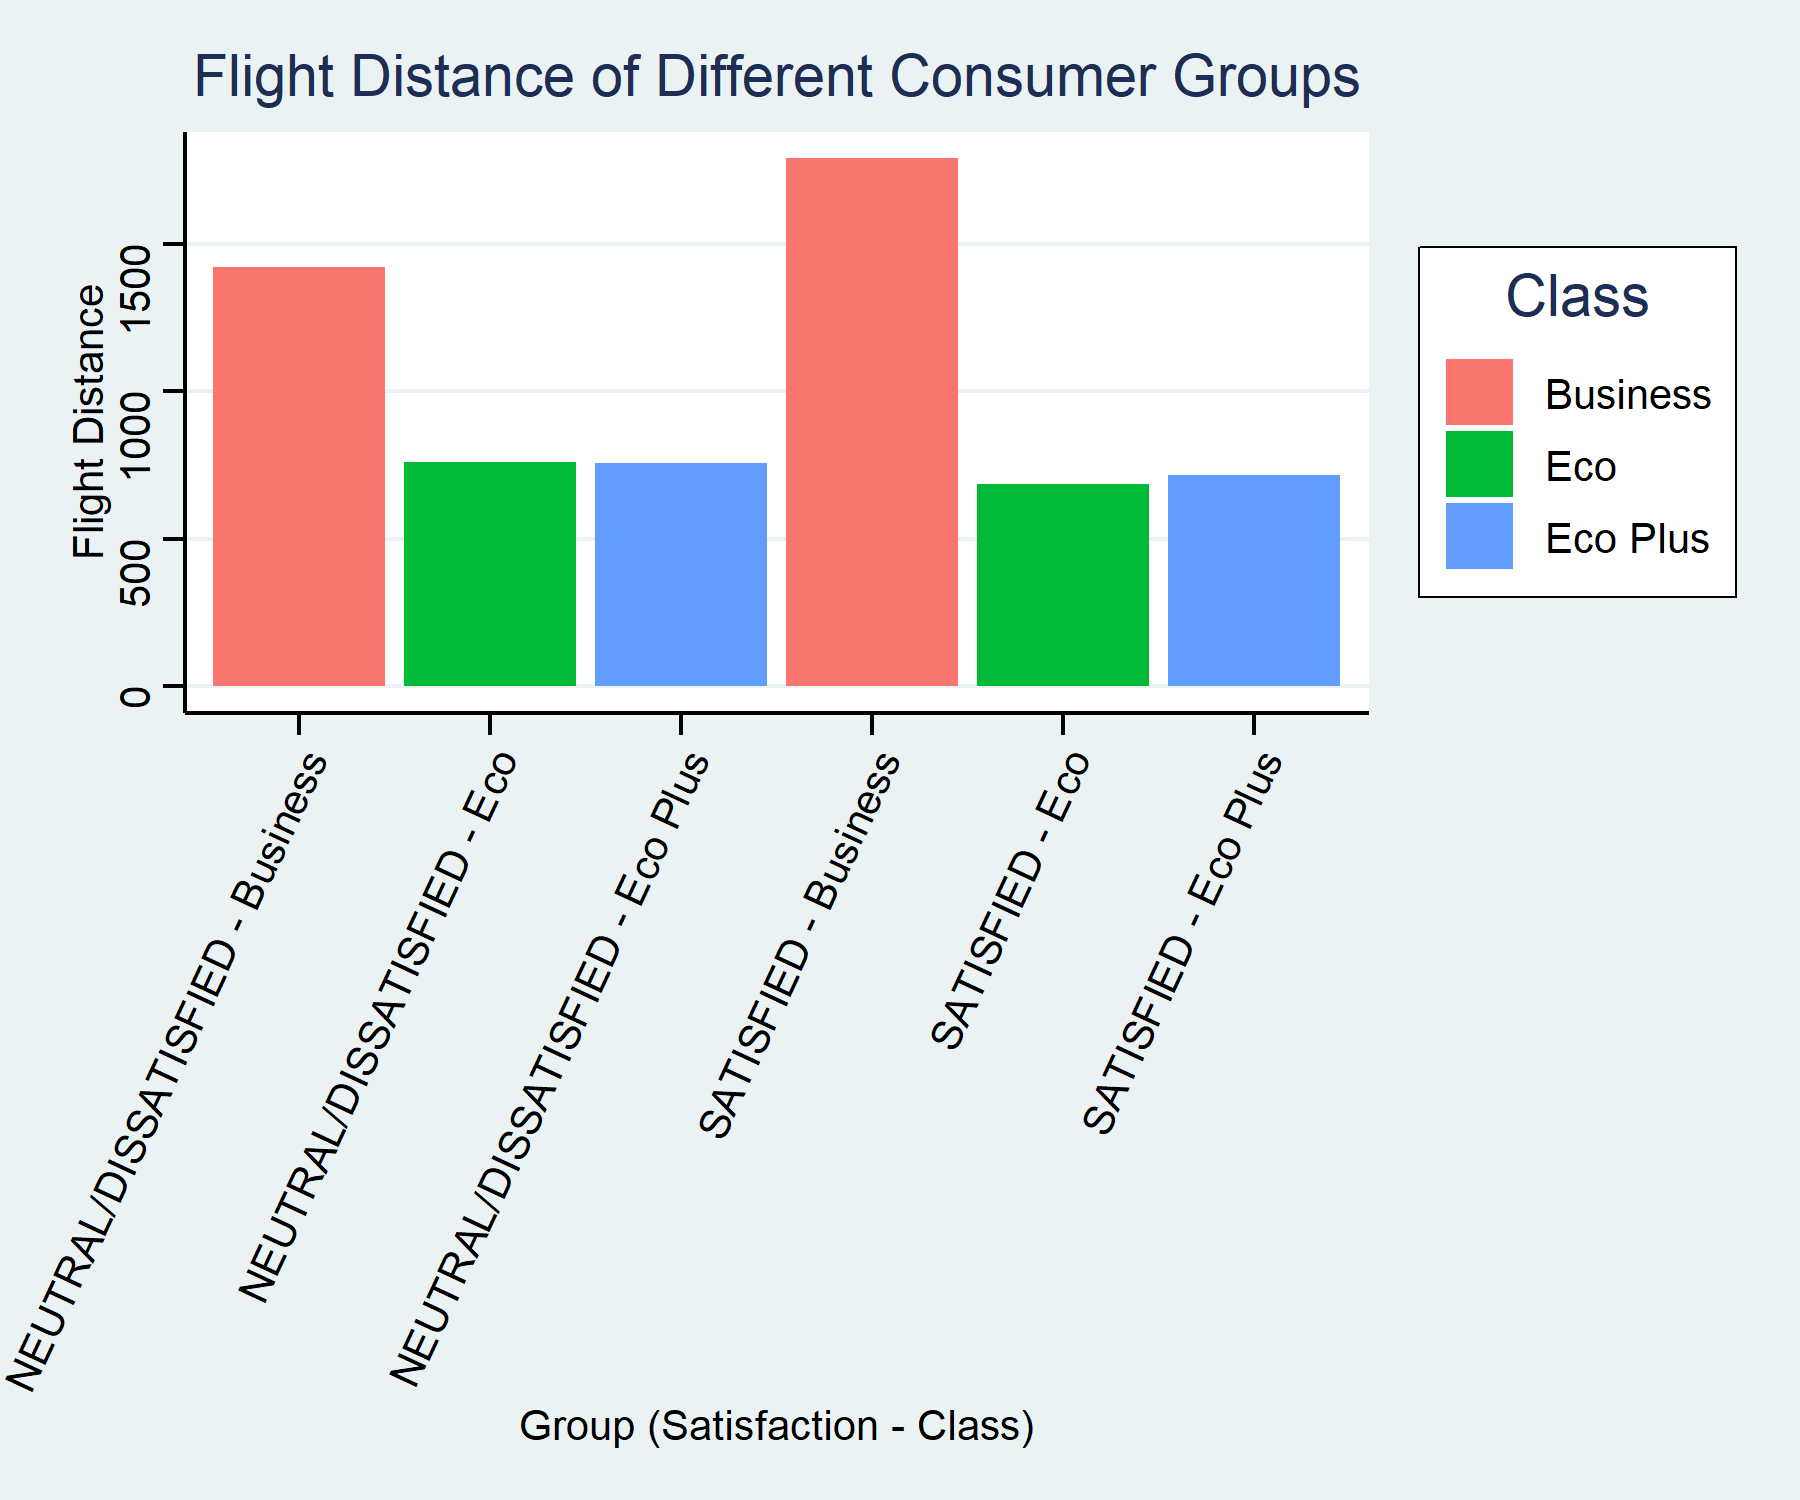
\includegraphics[width = 6in, height = 5in]{PS6b_DeVore.png}}\\
 \\
\noindent{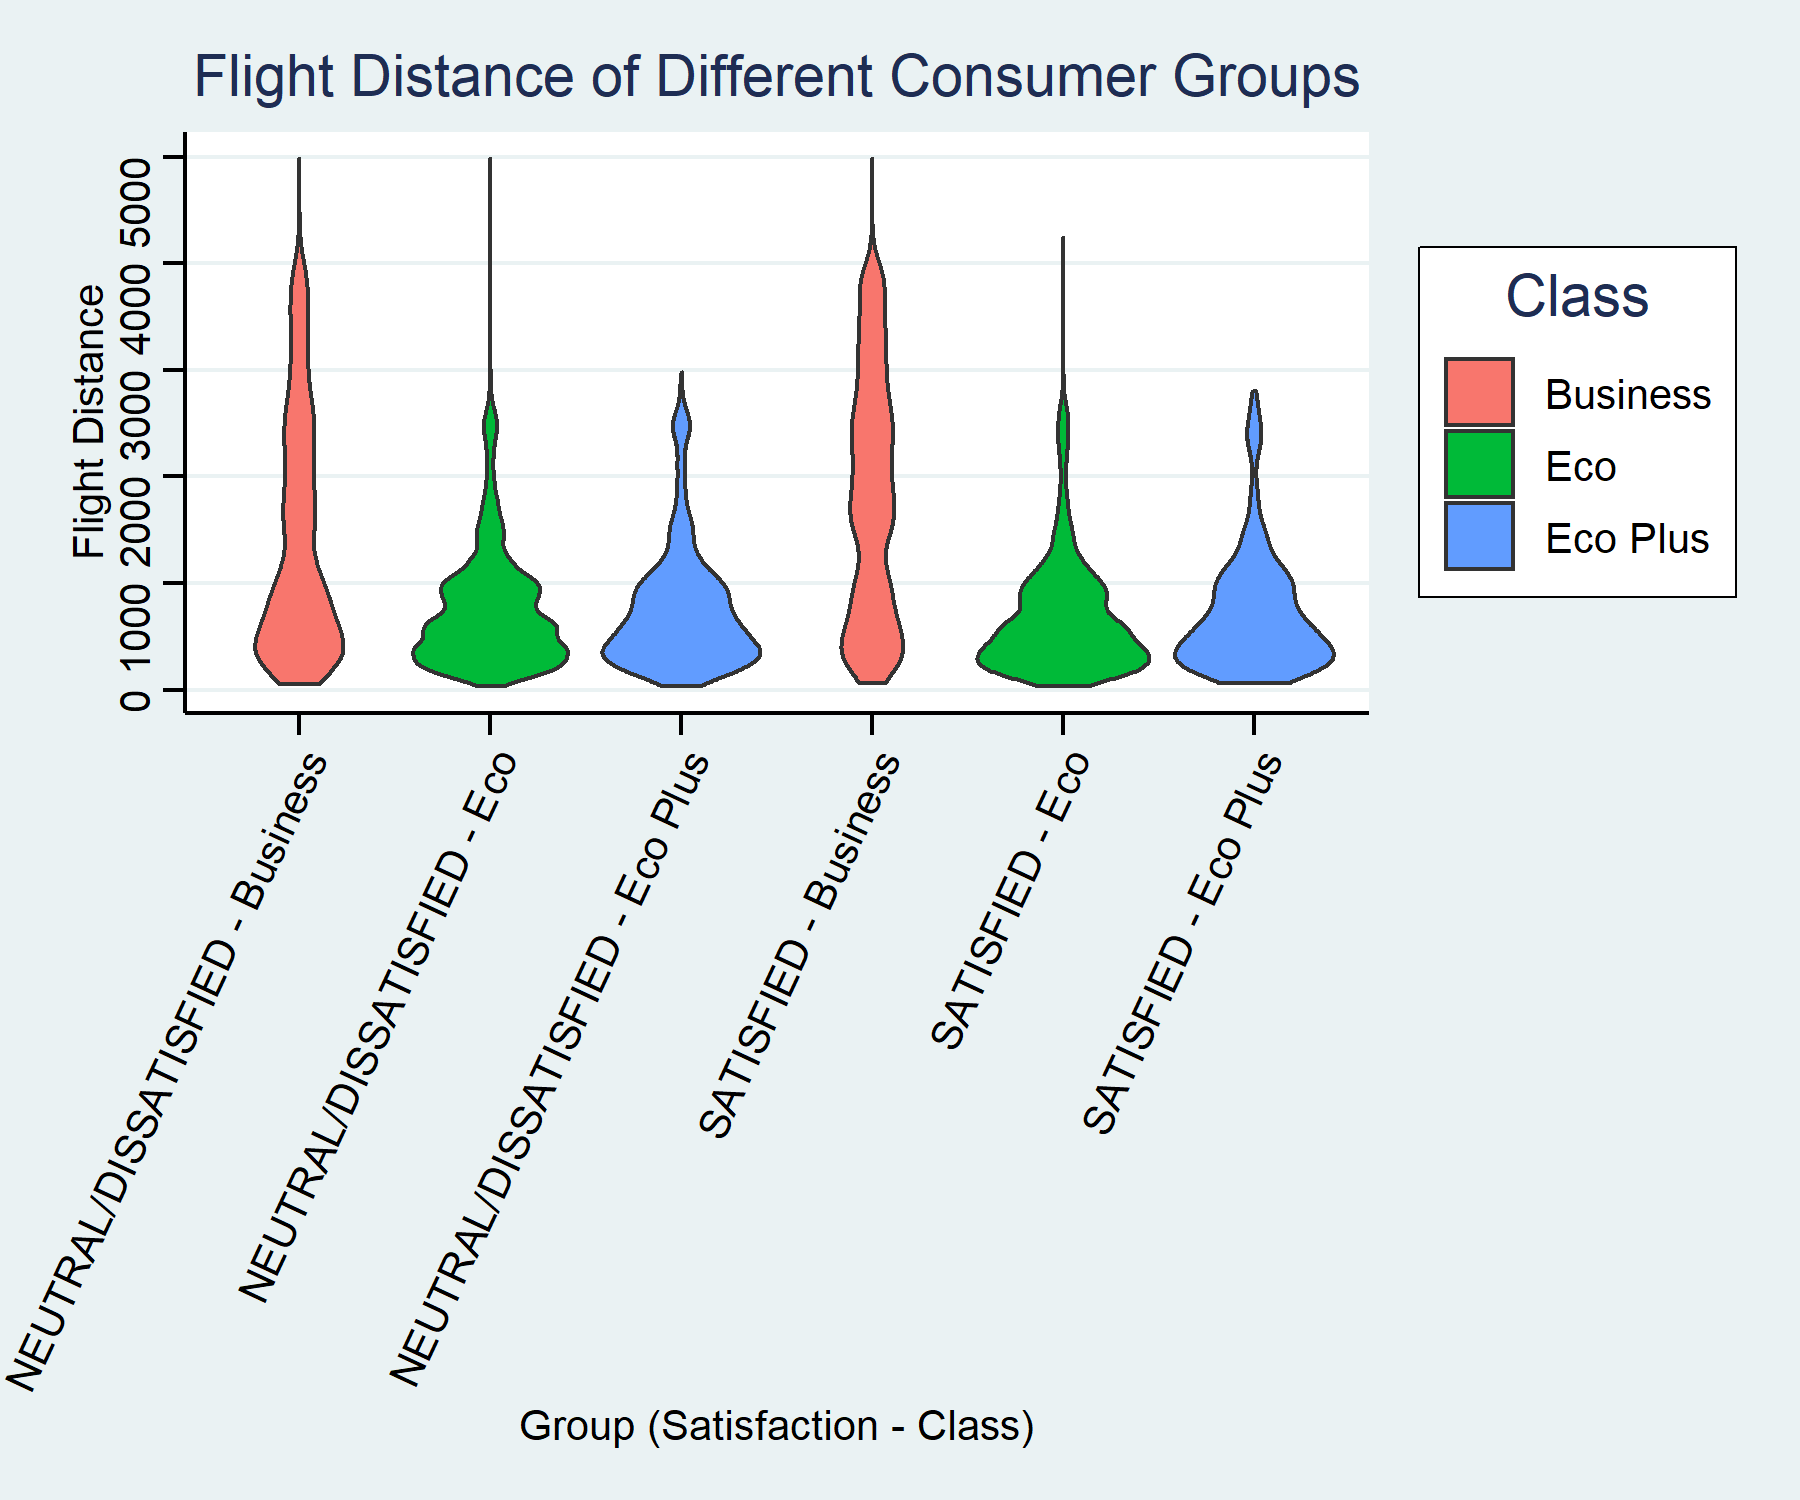
\includegraphics[width = 6in, height = 5in]{PS6c_DeVore.png}}\\
 \\

\newpage
\section*{Question 5}
\indent{The data I am using is chosen for experimental purposes. As such, I was able to make the first visualization, which I also made as a bit of an experiment. Though very basic in its current form, the first plot shows the satisfaction rate in a donut chart. 42.9\% of the individuals in the dataset report being satisfied, while 56.1\% report being either neutral or dissatisfied. These charts, of course, can become more complicated, but this should be sufficient for an introduction to the dataset.}\\
\indent{The second plot is a bar graph of the flight distance of the different satisfaction levels and cabin classes, where the color is sorted by classes so that they can be compared side-by-side. For the purposes of this analysis, the overall averages for each group are used. It is interesting to note that the farther a business class individual has to travel, the more likely they seem to be to report being satisfied. For the economy and economy plus classes, they seem to have the same opinion regardless of the distance flown.}\\
\indent{The final plot is similar to the second plot, however it uses a violin plot to show the distributions of the difference satisfaction levels and classes, rather than the averages. As stated in the previous graph, the economy and economy plus class seem to stay the about the same regardless of the flight distance. For the business class, however, it is thicker near the top, suggesting that individuals who have a longer flight distance are more likely to report being satisfied.}\\
\end{document}
